\documentclass[10pt,a4paper]{article}
\usepackage[utf8]{inputenc}
\usepackage[spanish]{babel}
\usepackage{amsmath}
\usepackage{amsfonts}
\usepackage{amssymb}
\usepackage{graphicx}
\usepackage{multicol}
\usepackage{titling}
\usepackage{titlesec}
\usepackage{array}
\usepackage{bm}
\usepackage{afterpage}
\usepackage{booktabs} %LIBRERIA PARA EXCE
\usepackage{multirow}
\usepackage{float}
\usepackage{pdfpages}
\usepackage{graphicx}
\usepackage{epstopdf}
\usepackage{longtable}
\usepackage{xcolor}
\usepackage[spanish]{babel}
\usepackage[utf8]{inputenc}
\usepackage[spanish]{babel}
\usepackage[utf8]{inputenc}
\usepackage{tikz}
\usepackage{verbatim}
\usepackage{smartdiagram}

\usepackage{multirow}


\usetikzlibrary{shapes,arrows}
\usepackage{color}
\usepackage{epigraph}
\setlength\epigraphwidth{1.5\textwidth}
\usepackage{subfigure}
\usepackage{anyfontsize}
\usepackage[left=2cm,right=2cm,top=2cm,bottom=2cm]{geometry}

\usepackage[colorlinks=true,
            linkcolor=blue,
            citecolor=blue,
            urlcolor=blue]{hyperref}

\begin{document}
\author{Chandi Armando} % CAMBIAR A AUTORES
\title{\textbf{PERCEPTRÓN DE UNA CAPA PARA PREDICCIÓN DE CALIDAD DEL AIRE}}
\date{17 de febrero de 2020}
\maketitle  

\section{Introdución}

Debidos a que la contaminación ambiental ha ido en auge constante debido a la industrialización, actualmente se registran daños ambientales en puntos o zonas especifica alrededor del planeta, causa por la cual hay grandes pérdidas tanto a nivel social, económico y disminución de espectativa de vida en la fauna mundial incluyendo al ser humano, por lo que se ha visto necesario realizar la implementación de un sistema que pueda medir la calidad del aire. El principal objetivo es realizar un análisis de la calidad del aire en varios puntos de muestreo considerados representativos para la obtención de datos de alta relevancia, reales, útiles y que presenten un margen de error mínimo con el fin de determinar comportamientos futuros. Uno de los principales métodos de solución que contribuyen a la determinación de la calidad del aire y efectos sobre la salud implica las redes inalámbricas con lectura de sensores, estos dispositivos inteligentes son capaces de detectar, almacenar y analizar los flujos de datos en una red de información y comunicación.\\
para la estimación de comportamiento futuros que determinen la calidad del aire se realiza un análisis a través del machine learning o aprendizaje de máquina, la cual es una disciplina científica de la inteligencia artificial que crea sistemas que aprenden automáticamente a través de la identificación de patrones en cientos o miles de datos, la máquina aprende un algoritmo que es capaz de definir los datos y predecir un comportamiento futuro; esta tecnología se encuentra en desarrollo exponencial dando lugar a constantes mejoras que permiten al sector empresarial adquirir estrategia de producción y ventas de productos o servicios a la vez que beneficios ambientales de acuerdo al tipo de mercado y proceso.\\
En el presente proyecto se implementa el algoritmo de una red neuronal simple conocida como perceptrón de una capa o perceptrón simple en un microcontrolador Arduino; esta red neuronal trabaja en base a muestras de componentes del aire como Humedad, Temperatura, concetración de partículas pm10, y concentración de rayos UV, a las cuales se les asigna un peso de impacto sobre una función de activación para determinar una predicción de la calidad del clima.\\


\section{Diseño del sistema}
\subsection{Placa del sistema}

Para el desarrollo de este proyecto se usará un microcontrolador WIFI ESP8266, en conjunto con sensores que permiten la captura de datos en el aire del medio ambiente, los cuales se interconectan para dar lugar al sistema final.
Los diferentes sensores son ensamblados en baquelita, posterior a un diseño circuital de las pistas que garanticen la conductividad correspondiente a cada uno de los dispositivos.

\subsection{Conexiones}

Se debe tener en cuenta el orden de conexiones de todos los dispositivos para el funcionamiento del sistema para ello se crea un previo diseño en el software libre Fritzing, el cual es un programa que permite hacer esquemas eléctricos, y diseñar esquemas PCB, a continuación se muestra el diagrama de conexiones del sistema. 

\begin{figure}[H]
\centering
 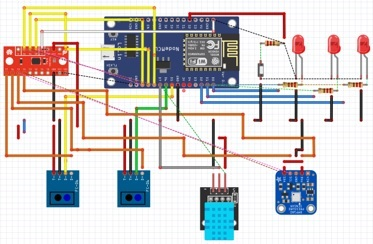
\includegraphics[scale=0.80]{fritzingcorregido.JPG} 
\caption{Diagrama de conexiones diseñado en Fritzing} 
\end{figure}

Las conexiones que se realizan constan de: tres leds con sus respectivas resistencias los cuales dan a conocer la interpretación de la calidad del aire en función a los datos de entrada , y los diferentes enlaces entre el microcontrolador MCU ESP8266 y los senspres MQ7, MQ135, DHT11,y el Sensor de Rayos UV GYM L8511

\subsection{Diagrama de conexión }

Para la realización del diagrama de pistas en la PCB, se utiliza el software PCB Wizard, el cual permite crear esquemas de circuitos electrónicos y a partir de estos, obtener de una manera sencilla el diseño del circuito impreso a una o dos caras.

\begin{figure}[H]
\centering
 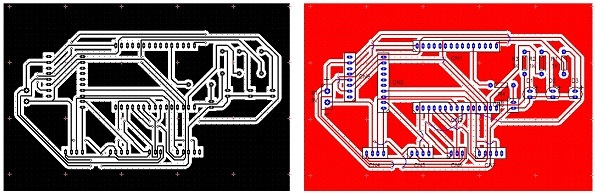
\includegraphics[scale=0.68]{placasensores.JPG} 
\caption{Pista esquemática PCB} 
\end{figure}

El proceso de fabricación de una placa PCB, se lo realiza con una impresión láser del circuito en papel couche, luego se lo recorta del tamaño necesario para la placa,consiguiente se planchar el recorte sobre la baquelita de cobre, permitiendo a la tinta a láser y el papel couche impregnarse en la placa por el calor; finalmente a la baquelita se lo pone ácido por unos minutos para que el cobre que no este cubierto por la tinta se elimine, quedando así las pistas conductoras de cobre. \\
A continuación de este proceso se realizan las perforaciones con taladro de broca delgada, teniendo cuidado que las pistas puedan ser afectadas.\\


\section{Desarrollo}

\subsection{Diagrama de Bloques del sistema}

\begin{figure}[H]
\centering
 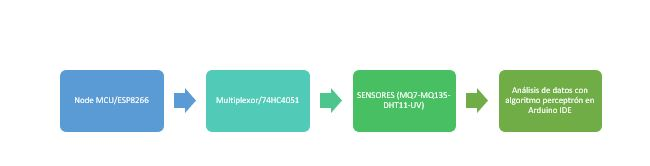
\includegraphics[scale=0.88]{bloques.JPG} 
\end{figure}

\subsection{Algoritmo Peceptrón}

El algoritmo perceptrón de una capa es un modelo unidireccional compuesto por una señal de entrada y una de salida, para el caso del análisis de datos capturados referentes a la calidad del aire los datos de entrada son la variables de humedad, pm10, p2.5 y concentración de rayos UV y los datos obtenidos a la salida son el resultado posterior a una función de activación denominada umbral en donde se determina un valor binario que se interpreta como aire no contaminado (1) y aire contaminado(0).\\
A continuación de da a conocer un diagrama de flujo del funcionamiento del sistema.\\
\begin{figure}[H]
\centering
 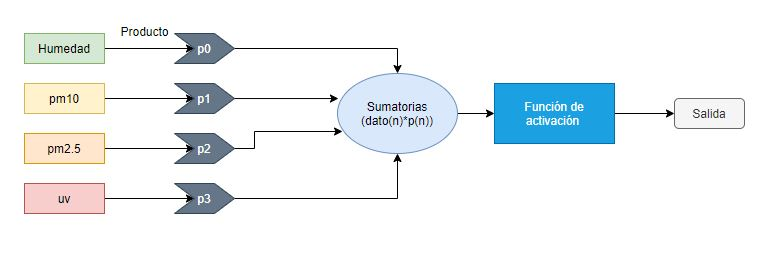
\includegraphics[scale=0.7]{bloquePerceptron.JPG} 
\end{figure}

\subsection{Selección de los sensores para toma de datos}

Para poder escoger entre estos sensores se procedió a comparar con varios tipos; existen diferentes opciones tanto genéricas como profesionales para efectos del proyecto serán necesarios sensores que puedan obtener datos de aire, humedad y temperatura.\\

\textbf{Placa NodeMCU}\\

Es un microcontrolador que trabaja bajo código abierto y esta basado en el chip ESP8266 (ESP-12E), que utiliza el lenguaje de programación Lua para crear un ambiente de desarrollo para aplicaciones que requiera conectividad Wifi de manera rápida.
El ESP8266 ofrece una solución completa y autónoma de redes Wi-Fi, lo que le permite alojar la aplicación o servir como puente entre Internet y un microcontrolador, tiene potentes capacidades a bordo de procesamiento y almacenamiento que le permiten integrarse con sensores y dispositivos específicos de aplicación.\\

\textbf{Sensor DHT-11}\\

El DHT11 es un sensor de humedad relativa y temperatura de bajo costo y de media precisión. Integra un sensor capacitivo de humedad y un termistor para medir el aire circundante, y muestra los datos mediante una señal digital en el pin de datos . \\

\textbf{Sensor MQ-7}\\

Este sensor es de alta sensibilidad al monóxido de carbono (CO), pero también es sensible al H2.  Puede detectar concentraciones en el rango de 20 a 2000ppm.
El módulo posee una salida analógica que proviene del divisor de voltaje que forma el sensor y una resistencia de carga. También tiene una salida digital que se calibra con un potenciómetro, esta salida tiene un led indicador.\\

\textbf{Sensor MQ-135}\\

Se utilizan en equipos de control de calidad del aire para edificios y oficinas, son adecuados para la detección de NH3, NOx, alcohol, benceno, humo, CO2, etc
Este sensor no proporciona valores absolutos, sino que simplemente proporciona una salida analógica que debe ser monitoreado y se comparada con los valores de umbral.\\

\textbf {Sensor Rayos UV GYML8511}

Este sensor UV, se utiliza para detectar el índice de intensidad ultravioleta (UV). Tiene una amplia gama espectral de 200nm hasta 370nm*. La señal eléctrica de salida del módulo es de tipo analógica, que varía respecto a la intensidad de los rayos \\

\section{Estimación de calidad del aire con algoritmo PERCEPTRÓN DE UNA CAPA }
\subsection{Captura de datos}

El sistema en funcionamiento permite realizar la captura de datos de humedad, temperatura, pm10, pm2.5 y concentración de rayos UV en tiempo real: la recepción de datos se puede visualizar en Arduino IDE a través de comunicación serial desde el ESP8266.\\

\begin{figure}[H]
\centering
 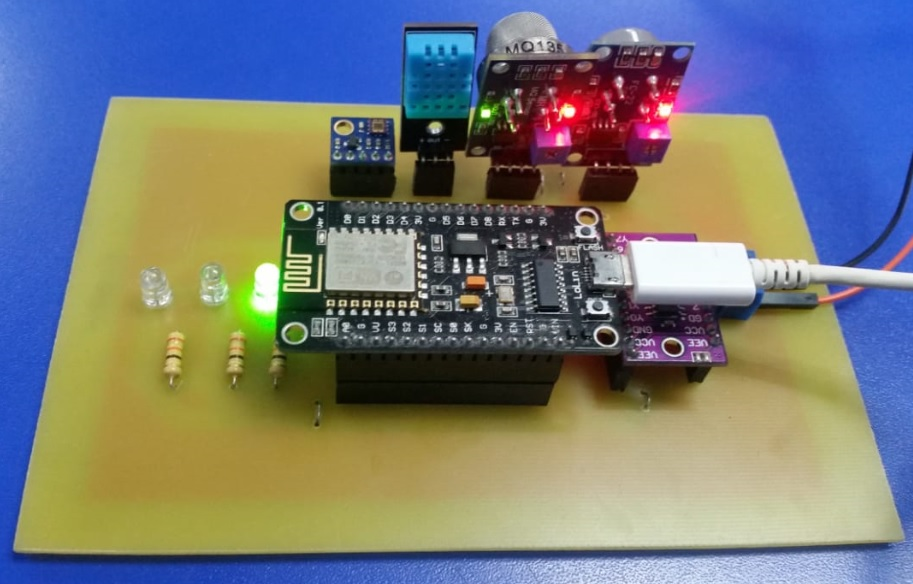
\includegraphics[scale=0.38]{placanueva1.JPG} 
\caption{Sistema en funcionamiento para captura de datos} 
\end{figure}

\subsection{Procedimientos en Rstudio}
Con el fin de crear una base de datos de entrenamiento y prueba a partir de una base de datos adquiridos en 2 diferentes ambientes; se utilizo Rstudio, un software que permite el análisis de datos a través de programación.\\

Para la determinación de los pesos de cada una de las variables sobre el sistema, se utiliza la librería Boruta, la cual permite graficar este método sobre un plano bidimensional en función de grado de importancia y atributos.\\

\begin{figure}[H]
\centering
 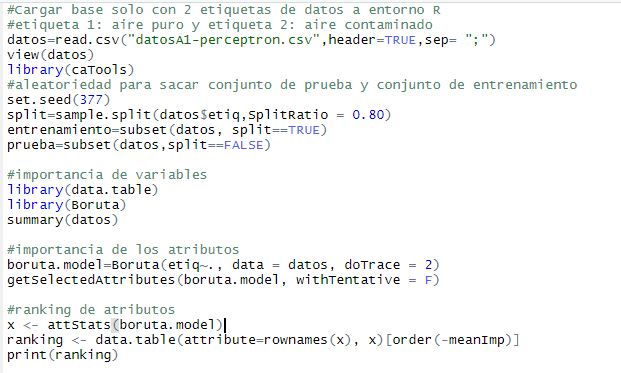
\includegraphics[scale=0.7]{codigoR.JPG} 
\caption{Código para selección de datos y pesos en Rstudio} 
\end{figure}

\begin{figure}[H]
\centering
 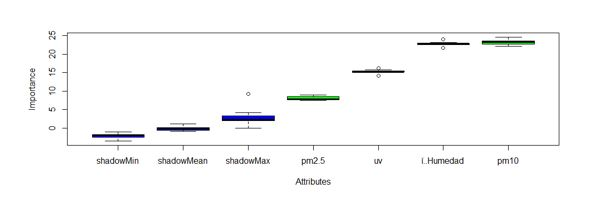
\includegraphics[scale=1]{importancia.JPG} 
\caption{Relación de relevancia de variables} 
\end{figure}
\subsection{Análisis de muestras con algoritmo Perceptrón desde Arduino IDE}

\begin{figure}[H]
\centering
 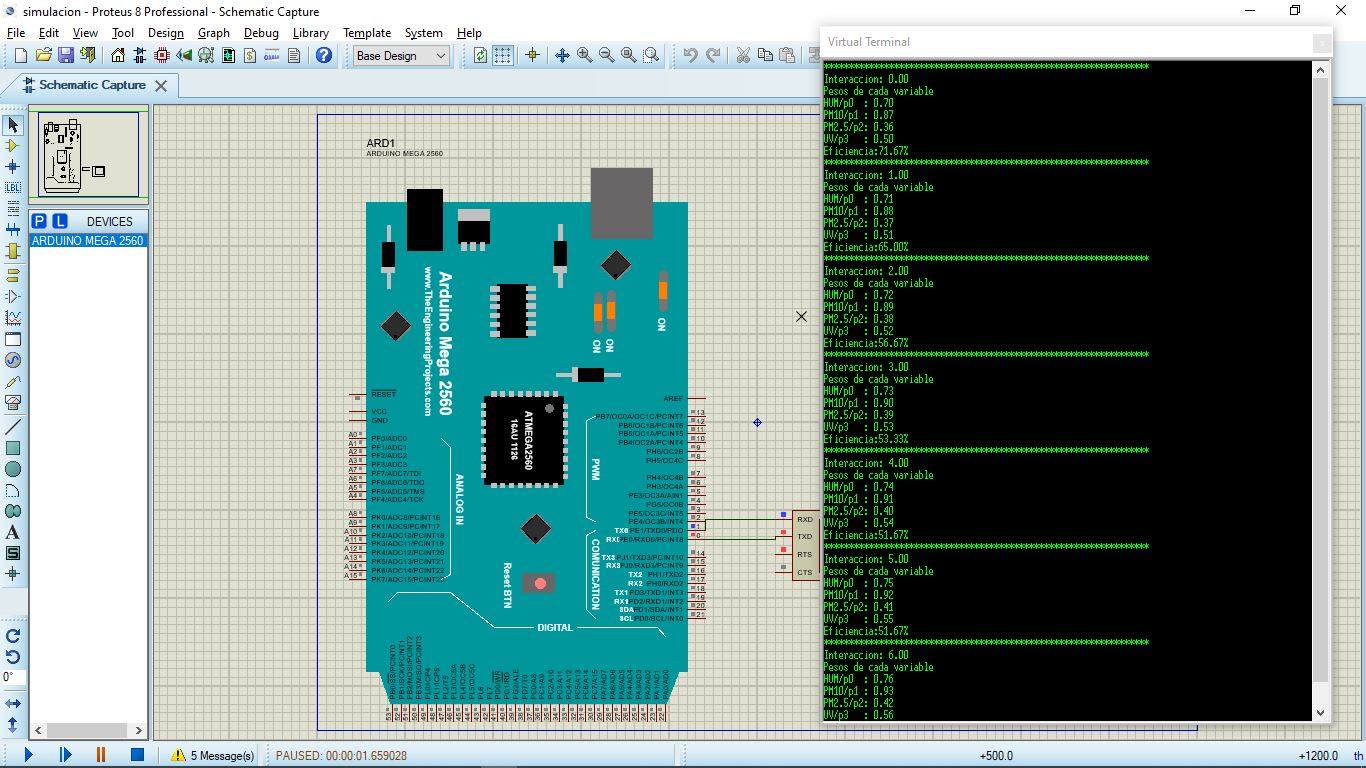
\includegraphics[scale=0.45]{simulacion.JPG} 
\caption{Simulación del algoritmo Perceptrón en Proteus con Arduino Mega} 
\end{figure}

El análisis de muestras se realizó en un algoritmo programado en Arduino IDE el cual se ejecuta en la placa Arduino Mega debido a la capacidad de procesamiento, para poder obtener resultados óptimos se asignó un peso a cada variable, el cual en constantes interacciones del sistema va variando con el fin de encontrar los pesos ideales que permiten garantizar la eficiencia del sistema y por ende de una predicción.

\section{Interfaz}

La interfaz fue diseñada con el objetivo de tener una mejor interacción entre el usuario y el prototipo, con el cual se ha creado de una manera dinámica en el que se podrá observar tanto los componentes contaminantes como el estado del ambiente que se analiza.\\

La plataforma esta constituida por dos botones: desconectar, será aquel que habilita el sistema para empezar a realizar el análisis; mientras que el botón guardar nos dará la opción de poder crear una tabla de los datos de los sensores para el estudio profundo con respecto a los contaminantes del aire. También se implementa un medidor de la calidad del aire siendo 0.0 puro y 5.0 contaminante.

\begin{figure}[H]
\centering
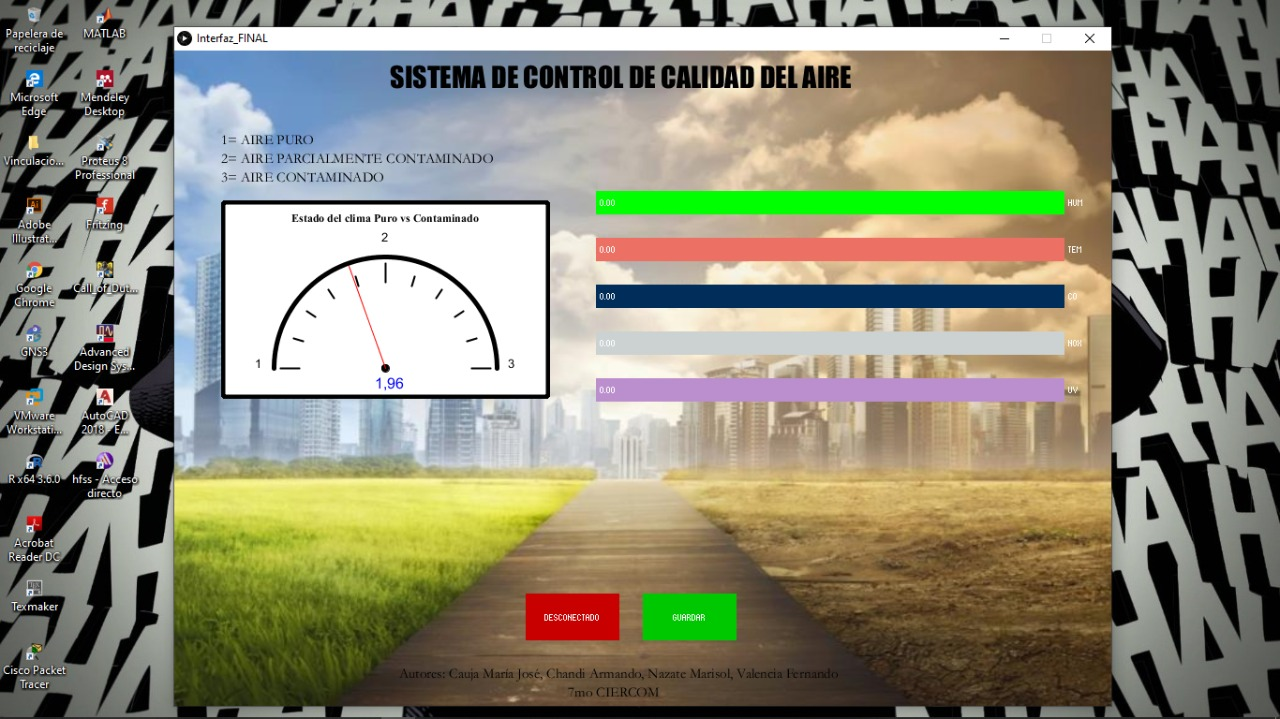
\includegraphics[scale=0.30]{interfaz.JPEG}
\caption{Interfaz} 
\end{figure}

\section{Conclusiones y Recomendaciones}
\subsection{Conclusiones}

El algoritmo perceptrón de una capa es conocido como el algoritmo mas básico de programación de una neurona y que permite que esta se entrene en función a un conjunto de datos en donde cada dato tiene un peso de impacto o peso relevante para la interpretación de futuros acontecimientos conocidos como predicciones.\\

Perceptrón de una capa necesita contar con pesos efectivos para garantizar el funcionamiento del sistema, para ello Rstudio puede ser un buen filtro ya que se puede relacionar el grado de relevancia de las variables con el peso que cada una tiene sobre la interpretación final de datos, caso contrario si se asignan pesos aleatorios se genera un margen de error en la función de activación, el cual impide que el sistema interprete los datos de entrada de forma correcta  \\

El software Rstudio permite la selección de datos de prueba y entrenamiento de forma aleatoria y su posterior interpretación de relevancia y ranking, se adquirió una base de datos de entrenamiento de 482 y de prueba de 120, pero el procesamiento de la placa arduino Mega es insuficiente así que de los datos de prueba se seleccionó al azar 120 datos de 2 etiquetas que determinan la calidad del aire como no contaminado (1) y contaminado(0).\\

El software de diseño Processing se basa en programación Java, C: y fue utilizado para la realización de una interfaz con enfoque a la oferta del servicio de evaluación de condición del clima para diferentes usuarios, esta interfaz se desarrolló con los componentes que la aplicación nos facilita.\\


\subsection{Recomendaciones}

Se debe calibrar los sensores de manera adecuada de acuerdo a la aplicación que se desea realizar y las necesidades del usuario.\\

La toma de datos debe ser de distintos ambientes, así se consideran las variaciones y el perceptron puede interpretar el dato. \\

El umbral en el cual la interpretación de datos de entrada da el salto de 0 a 1 debe ser considerado en función a los pesos efectivos de cada una de las variables, caso contrario el sistema sera ineficiente.\\ 

El diseño de una red neuronal de una capa da origen a una red multicapa la cual permite la evaluación de datos con probabilidades es por ellos que si se pretende trabajar a futuro bajo esta modalidad dentro de un sistema IoT se recomienda que el procesamiento que brinde el sistema garantice el flujo de datos por cientos o por miles.\\

\section{Anexos}

\begin{figure}[H]
\centering
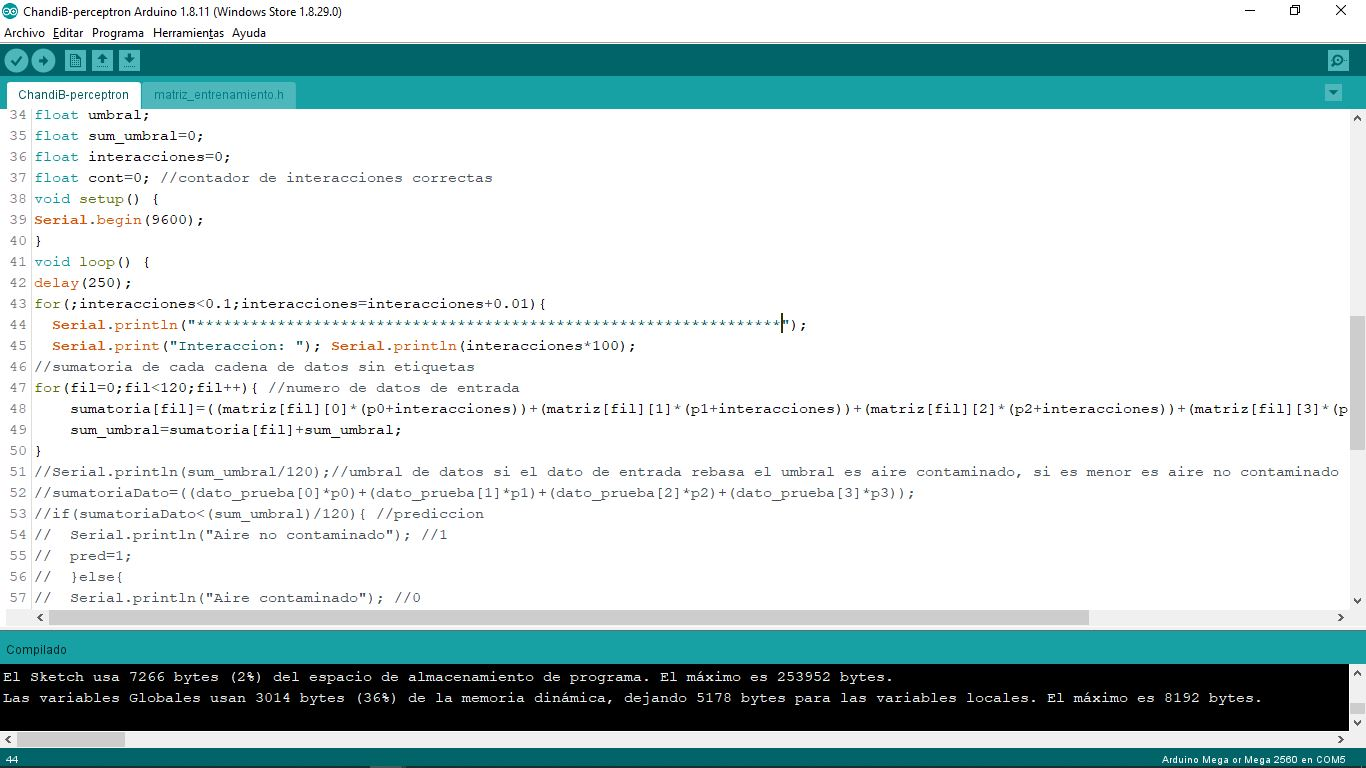
\includegraphics[scale=0.50]{pruebas.JPG}
\caption{Pruebas del algoritmo perceptrón realizadas desde Arduino IDE} 
\end{figure}



\end{document}
